\documentclass[border=3pt]{standalone}
\usepackage{tikz}
\usetikzlibrary{patterns}
\begin{document}
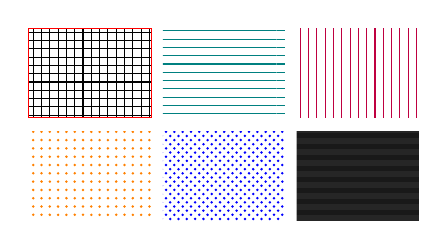
\begin{tikzpicture}
  \draw[draw=red,pattern=grid] (-.26,.13) rectangle (1.3,1.26);
  \fill[pattern=horizontal lines,pattern color=teal] (1.45,.13) rectangle (3,1.26);
  \fill[pattern=vertical lines,pattern color=purple] (3.15,.13) rectangle (4.7,1.26);
  \fill[pattern=dots,pattern color=orange] (-.26,-1.18) rectangle (1.3,-.05);
  \fill[pattern=crosshatch dots,pattern color=blue] (1.45,-1.18) rectangle (3,-.05);
  \fill[pattern=horizontal lines dark gray,pattern color=red] (3.15,-1.18) rectangle (4.7,-.05);
\end{tikzpicture}
\end{document}
